\subsection{Background}

The previous wing design team worked on developing a lightweight, manufacturable wings for the flyer and made several key contributions. In 2022, the team established an initial test framework by building a static deflection test stand capable of measuring deflection at 3 points (root, mid, and tip) along the span of the wing. This allowed for early comparison of different combinations of veins and membranes, and a database was created using the results obtained. In the static tests, the team explored a wide range of vein geometries and materials, including LW-PLA and PETG, with carbon fibre leading edge rods. The root control bar as designed by the flapping mechanism team in the same year was also incorporated in the wing.These efforts helped identify  structural issues such as excessive stiffness, excessive deformation at the trailing edge, and durability concerns. The final design was selected based on performance in the static tests and initial project requirements. 

Some work was done to characterize membrane materials such as polypropylene tape, Kapton, and RC covering film. The team observed that the membrane stiffness and vein geometry strongly influenced camber formation and overall deformation quality. Additionally, the team Identified root vein weaknesses. This revealed the need for reinforcement at the wing root to survive inertial loading at 30 Hz during stroke reversal.

Overall, a database of 12 prototype wings, documenting each design’s weight, geometry, and deformation profile was produced. Although static tests do not fully predict dynamic performance, the results helped in the selection of a wing design to compare results obtained this year to. The previous work also provided a foundation of viable materials and manufacturing processes for MFWF wings. These were used in the new prototypes developed this year. As the wing requirements remain the same this year, the insights from their work shaped this year’s focus on achieving controlled camber, improved stiffness gradients in vein geometry, and dynamic testing of new wing designs. The following are the requirements and constraints for the MFWF wing.

\begin{enumerate}
    \item The wing must be able to provide sufficient lift to the flyer.
    \item The wing must provide a means of attitude control via root actuation.
    \item To ensure the flyer is controllable, the wings must deform in a uniform and predictable manner.
    \item The wings must meet the following physical constraints
    \begin{enumerate}
        \item Each wing may have a span of up to 10 cm.
        \item Each wing can weigh up to 1.5 grams.
    \end{enumerate}
    \item The wing must be able to withstand the forces imparted on it for the duration of the flight. There are two peak loads of concern:
    \begin{enumerate}
        \item Peak inertial loads experienced during stroke reversal.
        \item Peak aerodynamic loads experienced at mid-stroke.
    \end{enumerate}
    \item The wings should be easy to manufacture and with consistent results.
\end{enumerate}

Figure \ref{fig:baselinewingmodified} shows the wing made of LW-PLA veins and Kapton tape designed by the previous teams. 

\begin{figure}[htb]
    \centering
    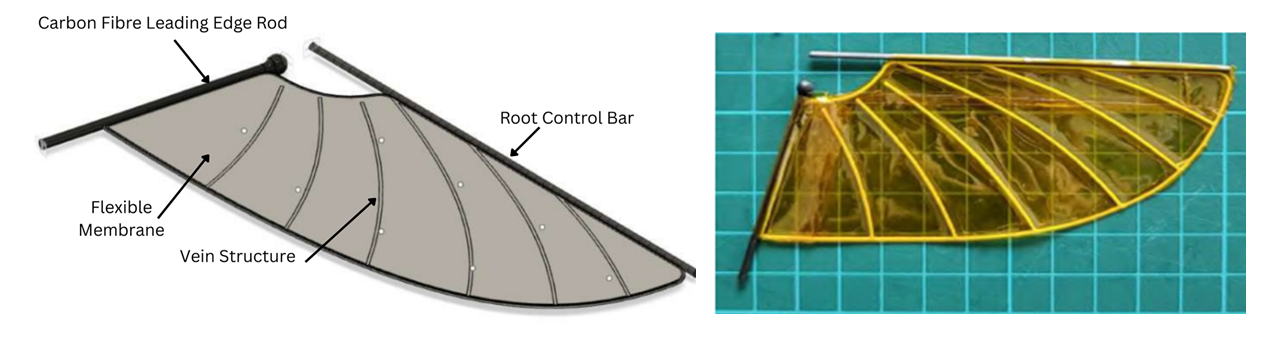
\includegraphics[height=4.5cm]{figures/baselinewingmodified.png}
    \caption{Baseline Wings: Final Wing Design from Previous Capstone Year \cite{MFWF_FinalReport2021}}
    \label{fig:baselinewingmodified}
\end{figure}

\subsection{Literature Review}

Building on insights from the 2021/22 and 2022/23 MFWF final reports~\cite{MFWF_FinalReport2021, MFWF_FinalReport2023}, a focused review of flapping-wing research was conducted to determine the deformation characteristics linked to efficient lift generation. The aim was to define an ``ideal'' deformation profile—specifically the combination of chordwise camber, passive twist, and spanwise bending observed in nature and flexible-wing FWMAVs. These characteristics directly inform the prototype designs developed this year. Figure \ref{fig:wingliftcharacteristics} shows important characteristics that contribute to a wings ability to generate lift. 

\begin{figure}[htb]
    \centering
    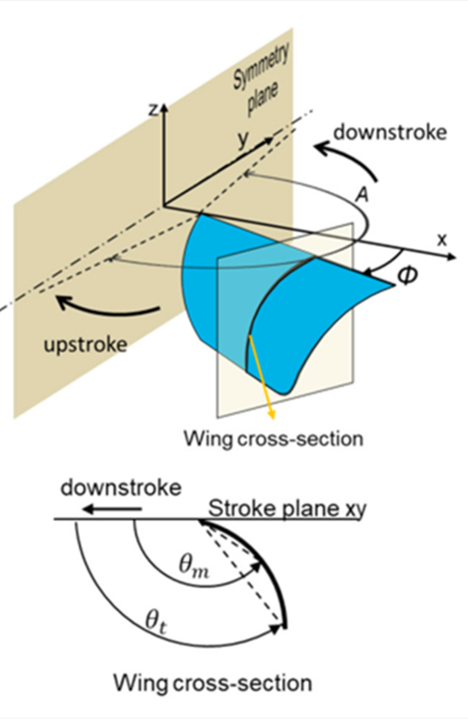
\includegraphics[height=6.5cm]{figures/wingliftcharacteristics.png}
    \caption{Wing Deformation Characteristics of a Flapping Wing \cite{dao2020corrugation}}
    \label{fig:wingliftcharacteristics}
\end{figure}

Most insect-scale flyers rely on passive aeroelastic deformation rather than rigid-wing aerodynamics\cite{ishihara}. Across beetles, flies, and insect-inspired robotic wings, three deformation modes consistently appear: camber, twist, and spanwise bending\cite{tian}. Chordwise camber between $5$--$12\%$ of chord was found to enhance the leading-edge vortex and increased lift during the power stroke\cite{wu}. Camber is evaluated using:
\begin{equation}
    f = \frac{h}{c},
\end{equation}
where $h$ is the maximum camber height and $c$ is the chord length. Thin membranes such as Mylar or polyurethane reliably achieve this camber range under aerodynamic loading.

Second, flexible wings typically exhibit $15^\circ$--$25^\circ$ of passive twist from root to tip~\cite{yoon,kraemer2012rapid}. The root follows the imposed motion while the tip lags due to lower torsional stiffness, shaping the leading edge vortex and improving downstroke lift. Third, insect wings bend downward by approximately $10$--$20\%$ of the semi-span under inertial loading~\cite{yoon}, aligning the wing with the local flow and reducing structural stress at flapping frequencies near 20--30 Hz.

Deformation also depends strongly on the interaction between veins and membrane stiffness~\cite{ishihara,kraemer2012rapid}. Intermediate veins help shape camber, a stiff leading edge maintains pitch at stroke reversal, and a compliant trailing edge supports both camber and twist.

\begin{table}[h]
\centering
\caption{Deformation characteristics for insect-scale flapping wings.}
\label{tab:ideal}
\begin{tabular}{l c l}
\hline
\textbf{Parameter} & \textbf{Target Range} & \textbf{Rationale} \\ \hline
Camber ratio $f = h/c$ & $5$--$12\%$ & Strong LEV and lift formation~\cite{wu,ishihara} \\
Passive twist & $15^\circ$--$25^\circ$ & Reduces tip stall; enhances downstroke lift~\cite{wu,kraemer2012rapid} \\
Spanwise bending & $10$--$20\%$ of semi-span & Aligns wing to flow; lowers stress~\cite{wu} \\
Membrane stiffness & Low--moderate & Allows smooth camber (Mylar, PP, PU) \\
Stiffness pattern & Stiff LE, flexible TE & Produces camber, twist, asymmetry~\cite{ishihara} \\ \hline
\end{tabular}
\end{table}

These deformation ranges define the criteria guiding this year's prototype development.It is important to note that these ranges are not idealized accross all flapping wings but specific wing architecture and geometries studied. Further experimentation will help identify an optimal range for the MFWF specifically based on flapping frequency, amplitude and lift force requirements. Variations in flexible membranes, vein geometry, and built-in camber were intentionally selected to evaluate how different structures reproduce these behaviours during the dynamic deflection tracking test.

\subsection{Design of Experiment}
A structured Design of Experiments (DOE) Table was developed to identify which wing architectures reproduce the similar deformation ranges established in the literature review. The DOE is fully defined, the baseline wing was remanufactured, an initial prototype set has been fabricated, and dynamic testing will proceed once the dynamic testing  setup is ready in the winter term. The objective is to determine how variations in membrane material and vein geometry influence camber, twist, and spanwise bending during flapping, while all other parameters remain same as in the baseline wing.

Following standard DOE principles, only a small set of variables are being varied, and all other conditions are held constant. The wings share a fixed span determined using the max span constraints mentioned earlier to ensure consistent inertial loading, while chord size, chord curvature, membrane choice, and vein geometry were selected as the experimental factors. This approach isolates the structural contributions of each design parameter, ensuring that observed differences in deformation can be attributed to controlled changes.

The prototypes span three built-in geometric camber levels (low, medium, high), implemented as camber angle extension to the membrane cutout, see Figure \ref{fig:camberangle}. 

\begin{figure}[htb]
    \centering
    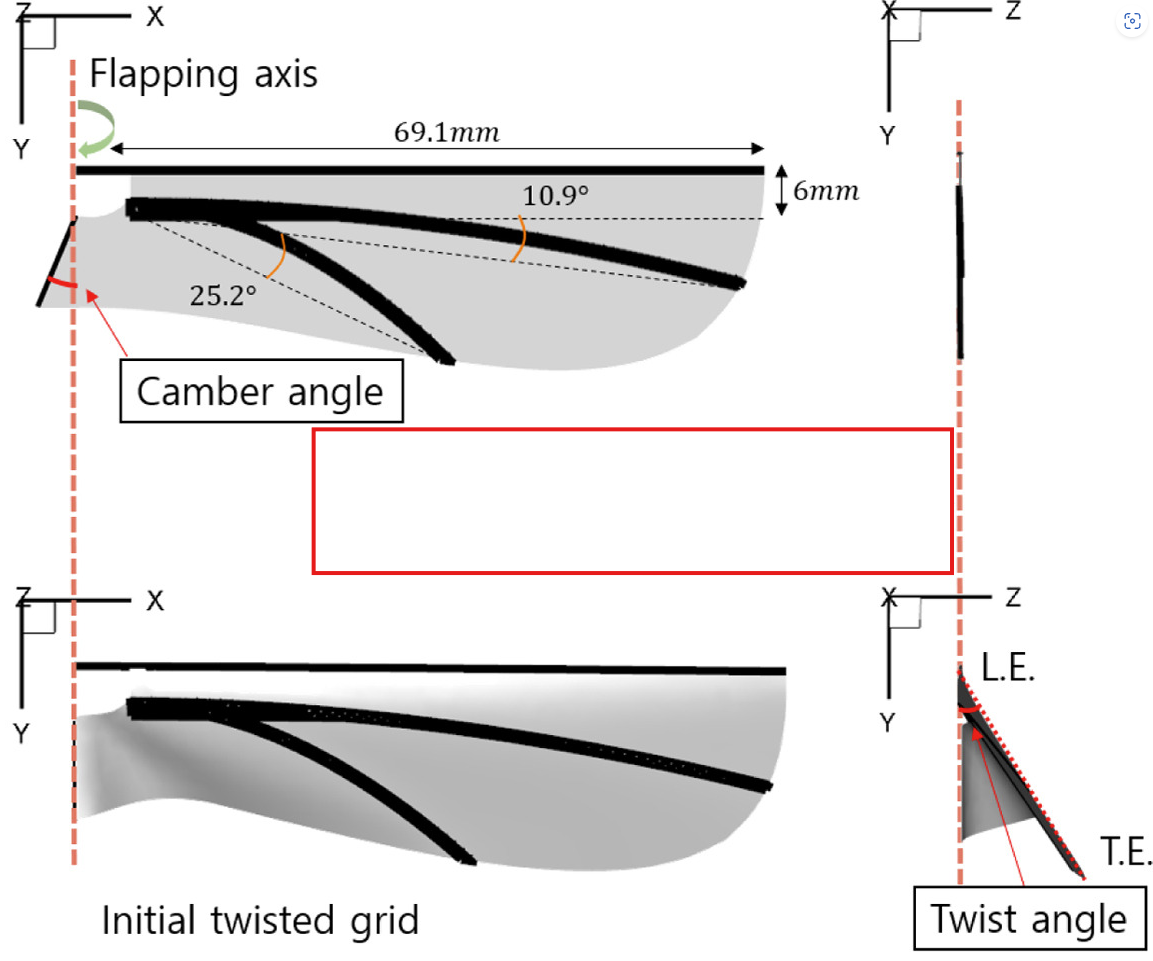
\includegraphics[height=6.5cm]{figures/camberangle.png}
    \caption{Camber Angle Extension and Twist Angle in Wing Design\cite{yoon}}
    \label{fig:camberangle}
\end{figure}

Membranes include polypropylene (PP) tape and Kapton, with Mylar included if available due to its favorable stiffness-to-weight properties. Vein geometry variations were introduced to shape chordwise flexibility and twist characteristics, including changes in vein stiffness and trailing-edge compliance.

All prototypes will undergo a dynamic deflection-tracking test and High-speed imaging will quantify deformation over the wingbeat cycle, including camber ratio and tip deflection as a measure of spanwise bending.

\begin{equation}
    f(t) = \frac{h(t)}{c},
\end{equation}
passive twist
\begin{equation}
    \theta_{\text{twist}}(t) = \theta_{\text{root}}(t) - \theta_{\text{tip}}(t),
\end{equation}

These quantities will be evaluated at mid-downstroke, stroke reversal, and mid-upstroke, allowing direct comparison to the ideal deformation targets reported for insect-scale wings.

The DOE provides a systematic and traceable framework for selecting the best-performing wing prototypes. Wings will be assessed on quantitative criteria: camber within $5$--$12\%$, twist between $15^\circ$ and $25^\circ$, spanwise bending within $10$--$20\%$ of the semi-span. A new wing variant with a modified leading-edge bar and control-bar geometry, introduced to meet the requirements of the electromagnetic flapping mechanism, will be evaluated under the same protocol. This experimental design ensures that the selected final wing is supported by measurable evidence and reflects the deformation behaviour of each wing prototype.

\begin{figure}[htb]
    \centering
    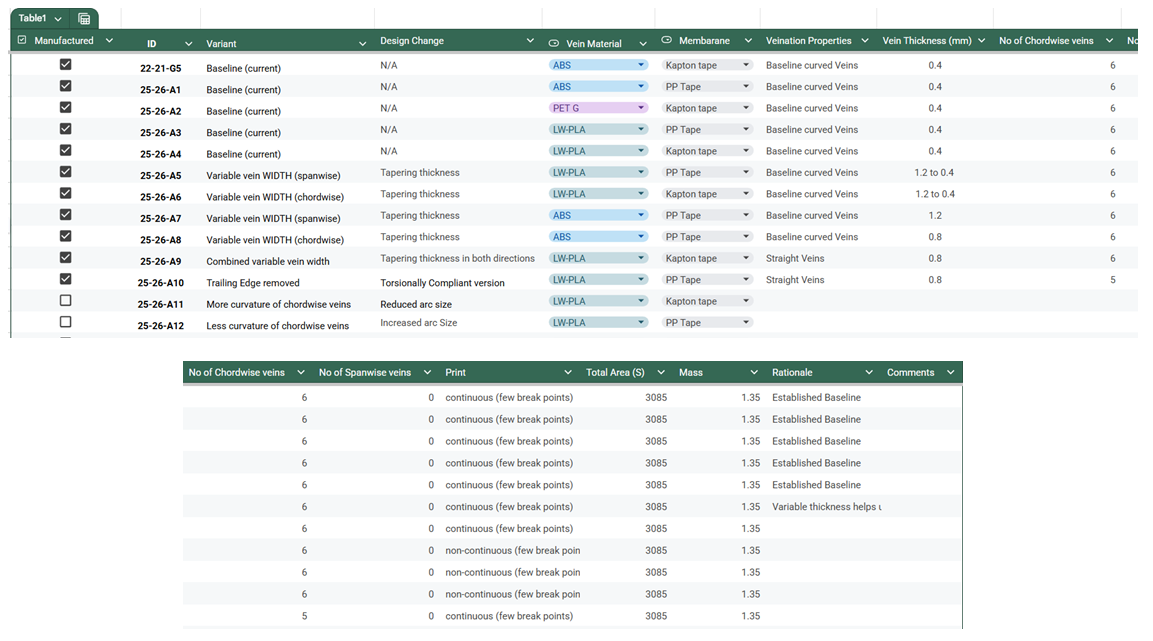
\includegraphics[height=9.5cm]{figures/doetable.png}
    \caption{Design of Experiments (Prototyping) Table }
    \label{fig:doetable}
\end{figure}
\subsection{Prototypes}
Prototyping this term focused on rebuilding a reliable set of baseline wings, and improving manufacturability. Since no testing has been conducted yet, all work centered on fabrication, refinement, and preparing the prototypes for testing. These tests will validate functionality of the prototypes

A major portion of the effort involved remanufacturing the baseline wing used in previous years. Early prints showed issues with vein thickness uniformity, and bubbles in the tape membrane. The baseline design was therefore modified to introduce curved edges, reprinted multiple times, with adjustments to print orientation, support strategy, and extrusion temperature. These changes resulted in improved prints.

\begin{figure}[htb]
    \centering
    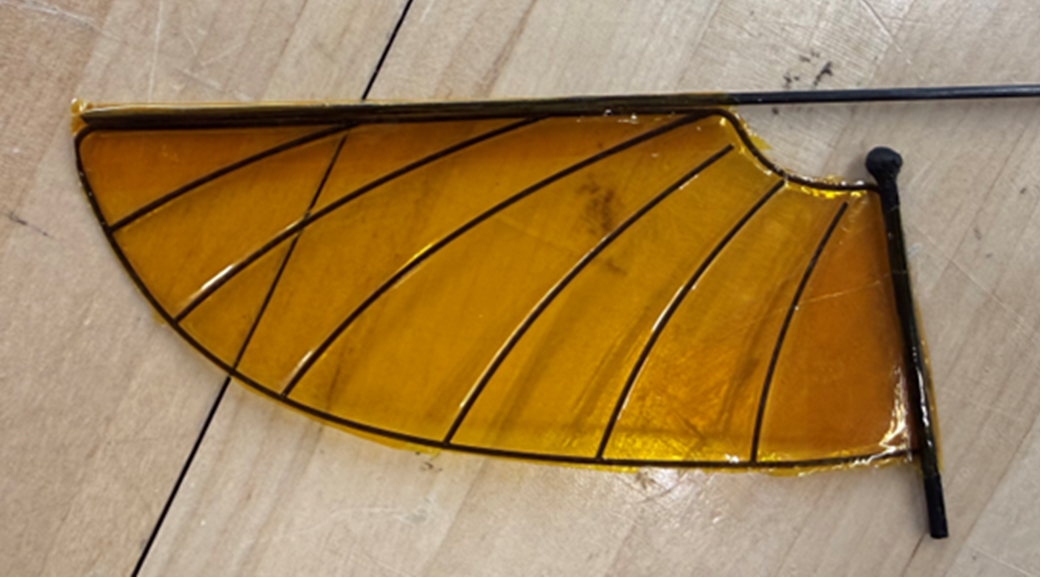
\includegraphics[height=4.5cm]{figures/newlymanufacturedwing.png}
    \caption{Baseline Wing Remanufactured with PETG Veins}
    \label{fig:newlymanufacturedwing}
\end{figure}

Beyond reproducing past work, the baseline geometry was also modified to improve fatigue resistance. Thin regions near the root and trailing edge experienced cracking during handling, indicating insufficient durability for prolonged dynamic motion. Local sharp internal corners were smoothed, and vein intersections were thickened slightly to distribute cyclic loads more evenly. These small geometric changes preserve the aeroelastic behaviour of the original design while significantly increasing the wing’s operational lifespan.

\begin{figure}[htb]
    \centering
    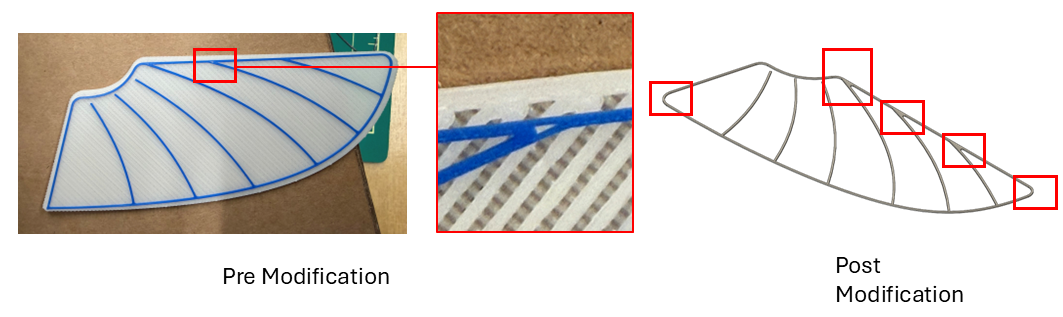
\includegraphics[height=4.5cm]{figures/baselinedesignchanges.png}
    \caption{Design Changes to Improve the Baseline Wing}
    \label{fig:baselinedesignchanges}
\end{figure}

A substantial amount of time went into resolving 3D-printing issues. LW-PLA required careful tuning to avoid voiding, layer delamination, and uncontrolled expansion. Several prints failed due to nozzle clogging, inconsistent extrusion, and instability when printing thin trailing edge veins for some prototypes. Adjustments included slowing down perimeter speeds, and increasing bed adhesion using custom brims. Printer calibration also had to be redone to correct some of these issues.

Once the baseline was manufactured successfully, attention shifted towards designing new wings that span the design variations outlined in the DOE. Multiple prototypes were fabricated with different chord sizes, built-in camber levels (low, medium, high), membrane materials (PP and Kapton), and vein geometries, see Figure \ref{fig:prototypes}. The 3D printed veins shown in Figure \ref{fig:prototypes} were not fully manufactured at the end of the term due to uncertainty in the interface between the the control bar and our test flapper, as the team is unsure what mechanism will be ready in time for the dynamic wing test. 

\begin{figure}[htb]
    \centering
    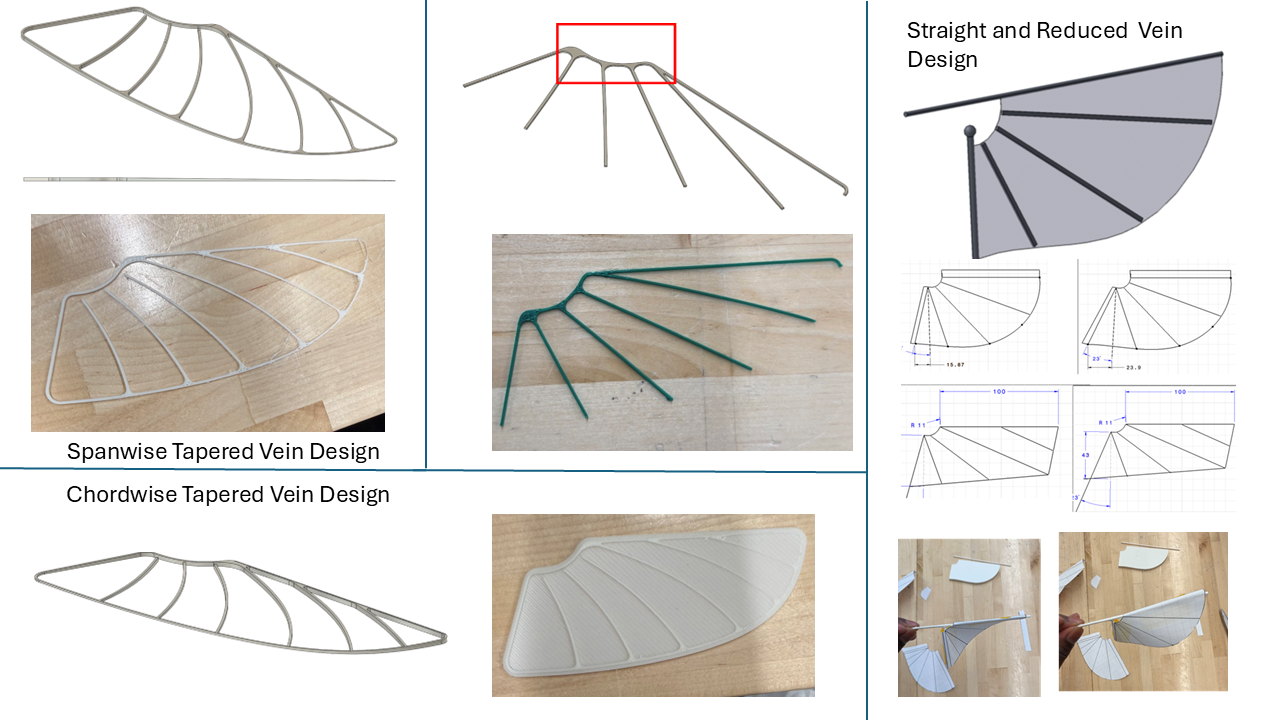
\includegraphics[height=6.5cm]{figures/prototypes.png}
    \caption{Design Changes to Improve the baseline Wing}
    \label{fig:prototypes}
\end{figure}

The final prototyping task involved modifying the leading-edge bar and control-bar design. This change was required after the decision to remove twist modulation by the electromagnetic flapping-mechanism team. Their system demands a different interface that can deliver the same stiffness near the root. The updated control bar and leading edge rod design improves load transfer into the wing, and ensures compatibility with the actuator’s stroke pattern. This modified bar will be used for all wings intended for dynamic testing next term. A more detailed version made of carbon fibre will be fabricated once interface decisions have been agreed on my the two teams during the winter term.

\begin{figure}[htb]
    \centering
    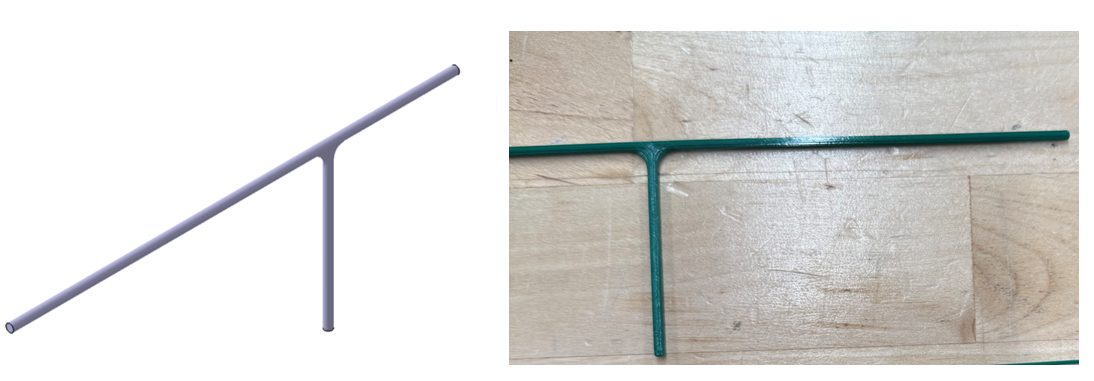
\includegraphics[height=4.5cm]{figures/controlbar.png}
    \caption{Preliminary Control Bar for testing}
    \label{fig:controlbar}
\end{figure}

\subsection{Plan for Winter Semester}
Work in the winter semester will focus on analysing the results from dynamic deflection-tracking tests and comparing the measured wing deformation to the ranges reported in the literature. From the high-speed recordings, quantitative metrics such as instantaneous camber ratio, root-to-tip twist, and spanwise bending amplitude will be extracted across multiple points in the flapping cycle. Additional timing data, such as phase lag between the leading edge and trailing edge, will help identify whether a wing responds too stiffly or too softly under dynamic loading. These measurements will directly inform the next round of prototypes by identifying which vein geometries or membrane materials produce desirable deformation patterns and which designs deviate from expected behaviour. Wings that demonstrate controlled camber formation, smooth passive twist, and repeatable bending profiles will be refined and re-printed for aerodynamic lift testing. 
In parallel, remaining interface questions with the electromagnetic flapping-mechanism team will be finalized to ensure that the revised leading-edge bar and control-bar designs integrate cleanly with their actuation system. Together, this work will establish a clear deformation-based selection pathway for the prototypes proceeding to aerodynamic evaluation.